\documentclass[12pt, letterpaper, twocolumn]{article}
\usepackage[margin=1.0in]{geometry}
\usepackage{graphicx}
\usepackage{float}
\usepackage{amsmath}
\usepackage{booktabs}
\usepackage{multirow}
\usepackage{tabularx,siunitx}
\usepackage[skip=0.5\baselineskip]{caption}
\usepackage{newtxtext,newtxmath}
\usepackage[autostyle]{csquotes}
\usepackage[most]{tcolorbox}
\usepackage{lipsum}
\usepackage[backend=biber,
    bibencoding=utf8,
    style=authoryear-icomp,
    sortlocale=de_DE,
    natbib=true,
    url=false,
    doi=true,
    eprint=false]{biblatex}
\usepackage[]{hyperref}
\hypersetup{
    colorlinks=true,
}
\addbibresource{references.bib}
\setlength{\headheight}{14.5pt}
%Handy Shortcut Macros
\newcommand\mX[1]{\multicolumn{1}{X}{#1}}
\newcommand\mcc[1]{\multicolumn{2}{c}{#1}}
\newcommand\mcl[1]{\multicolumn{2}{l}{#1}}
%Title Set Up
\title{Geometric Modeling of Gamma Coincidence}
\author{Austin Smith, Jordan Sturdivant, and Rahul Mehta\\
Department of Physics \& Astronomy, University of Central Arkansas
}
\date{}
% Document Beginning
\begin{document}
\frenchspacing
%Title Inserion
\maketitle{}
% Introduction
\section{Introduction}
A common nuclear process seen in radioactive sources involves the emission of
two gamma rays in coincidence (simultaneously). A source that undergoes this
phenomenon frequently is \textsuperscript{22}Na. \textsuperscript{22}Na exhibits
this process through $\beta$+ decay producing a positronium (positron electron
pair) which annihilates, emitting two gamma rays. These gamma rays in theory
have equal energies of 511 keV and a net momentum that is conserved. The
momentum of the positronium on paper is zero, therefore the direction of each
photon should be 180 degrees from the other to conserve momentum. The goal of
this experiment is too prove the angular correlation between these two
coincident gammas.
%Methods
\section{Method}
The angle of correlation between the coincident gammas, in theory is 180
degrees. This experiment tested this theory through comparing two different
models: the amount of coincidence counted at a given off-set (measured from
180 degrees) angle and a theoretical geometric model of coincident gammas with
180 degree correlation. The general design of the experiment involved two
gamma-ray detectors in a time-gate circuitry wired to only measure gammas that
hit both detectors within a short period of time between the other (Figure
\ref{figure:circuitry}). These detectors were set equidistant (varied from 15 cm
to 30 cm) from a source of NA-22 where one detector was held still, while the
other was rotated freely around the source (Figure \ref{figure:set_up}).
For the first model the angle of the detector was varied in increments of 1-2
degrees offset from 180 and a spectrum of coincident gamma rays was collected
for 120-240 second at each angle. This spectrum was integrated for each angle
to get the desired net count rate (Figure \ref{figure:spectrum}).
The second model aims to compares the overlapping area between detectors with
the net count rate per angle. If coincident gammas eject directly opposite from
each other, in order for any coincidence to be measured, part of the face of
each detector must overlap the other. This is essentially a measure of the
set-ups ability to count coincidence and the general trend can be compared with
the first set of data to see if the theory is supported.
%Results
\section{Results}
Table \ref{table:model1_table} diplays the measured count rates at their
respective offset angles from 180 degrees. The trend turned out to be similar
for both distances from the source showing a maximum count rate somewhere
between -1 to 1 degrees, and following a Gaussian curve as the offset angle
increased from the 180 degree angle. (Figure \ref{figure:model1_graph}).
For the second model, the overlapping area of the detectors as a function of
off-set angle, the geometry in Figure \ref{figure:geometry} was used. To start
this derivation, the the total area overlapped was set as a linear combination
of the area of the two inner circles $A_{1}$ \& $A_{2}$ (Figure
\ref{figure:geometry}). The areas of these pieces follow as:
%Equation Blocks
\begin{equation}
  \begin{gathered}
   A_{1} = 2\int_{d1}^{r1}\sqrt{r_{1}^{2}-x^{2}}dx \nonumber\\
   A_{2} = 2\int_{d-r_{2}}^{d1}\sqrt{r_{2}^{2}-(x-d)^{2}}dx \nonumber
  \end{gathered}
\end{equation}
After substitution and simplification we are left with:
\begin{equation}
  \begin{aligned}
  A_{total}=r_{1}^{2}cos^{-1}(\frac{d_{1}}{r_{1}})−d_{1}\sqrt{r_{1}^{2}−d_{1}^
  {2}}\\+r_{2}^{2}cos^{-1}(\frac{d_{2}}{r_{2}})−d_{2}\sqrt{r_{2}^{2}−d_{2}^{2}}
  \nonumber
  \end{aligned}
\end{equation}
where...
\begin{equation}
  \begin{aligned}
  d_{1} = \frac{r_{1}^{2}-r_{2}^{2}+d^{2}}{2d} \nonumber \\ d_{2} =
  \frac{r_{2}^{2}-r_{1}^{2}+d^{2}}{2d} \nonumber \\ d = \imath \cdot sin(\theta)
  \end{aligned}
\end{equation}
This formula only holds true for when $r_{1}\geq r_{2}$ and $d \geq r_{2} -
r_{1}$. Assertion 1 is always true in our set-up, however due to Assertion 2,
the correlation falls apart when the offset angle from 180 degrees is small.
These points were simply calculated at the area of the detector of smaller radius.
Once all of the overlapping areas were calculated (Table
\ref{table:model2_table}), we plotted and also fit the data with a Gaussian
function. While the fit had a bad confidence interval, the correlation between
the two models doesn't hinge on direct correlation. The fact that both sets of
data follow the general trend of having a maximum at 0 degrees, and a steep decrease
in area as the angle sweeps in either direction from this maximum, is enough to
point towards a 180 degree correlation. (Figure \ref{figure:model1_graph} and
\ref{figure:model2_graph}).
% Conclusion
\section{Conclusion}
While there is no strong correlation between the two models, the fact that
both models can even be fitted by the same function and follow the same shape,
is good evidence that there is a 180 degree correlation between gamma rays.
While this analysis doesn't prove without a doubt that the angular correlation
is always 180 degrees, it does fall in line with the narrative hypothesiszed.
Due to the conservation of momentum and the data collected, it is very likely
the correlated angle between coincident gamma rays is 180 degrees.

\newpage

\section{Figures and Tables}
%Table 1 of Coincidence Data
\begin{table}[H]
\centering
\begin{tabular}{ccccc}
\toprule
{Angles} & \multicolumn{4}{c}{Distance}\\\cmidrule{2-5}
& \mcc{\textbf{15 cm}}
& \mcc{\textbf{30 cm}}\\
\cmidrule{2-3} \cmidrule{4-5}
& {(+)}  & {(-)} & {(+)} & {(-)} \\
\midrule
12 & 0.10 & 1.82 & 0.10 & 1.46\\\hline
10 & 4.53 & 6.61 & 1.02 & 3.02\\\hline
8 & 17.66 & 16.09 & 1.84 & 5.63\\\hline
6 & 31.69 & 30.57 & 4.46 & 7.53\\\hline
5 & 37.70 & 33.87 & 5.16 & 9.26\\\hline
4 & 37.08 & 30.81 & 8.32 & 9.41\\\hline
3 & 40.90 & 37.20 & 9.13 & 9.77\\\hline
2 & 43.21 & 40.98 & 9.67 & 10.23\\\hline
1 & 42.67 & 40.22 & 10.02 & 10.10\\\hline
0 & 41.33 & 41.33 & 11.47 & 11.47\\\hline
\bottomrule
\end{tabular}
\caption{Measured coincidence data (counts per second) at varied offset angles
(degrees) and distances. In correspondance with model 1.}
\label{table:model1_table}
\end{table}
%Table 2 of Overlapping Area Data
\begin{table}[H]
\centering
\begin{tabular}{ccccc}
\toprule
{Angles} & \multicolumn{4}{c}{Distance}\\\cmidrule{2-5}
& \mcc{\textbf{15 cm}}
& \mcc{\textbf{30 cm}}\\
\cmidrule{2-3} \cmidrule{4-5}
& {(+)}  & {(-)} & {(+)} & {(-)} \\
\midrule
12 & 27.79 & 27.79 & 6.70 & 6.70\\\hline
10 & 31.96 & 31.96 & 13.01 & 13.01\\\hline
8 & 39.26 & 39.26 & 25.87 & 25.87\\\hline
6 & 40.41 & 40.41 & 28.05 & 28.05\\\hline
5 & 42.53 & 42.53 & 32.12 & 32.12\\\hline
4 & 44.63 & 44.63 & 36.26 & 36.26\\\hline
3 & 46.70 & 46.70 & 40.25 & 40.25\\\hline
2 & 48.68 & 48.68 & 44.64 & 44.64\\\hline
1 & 50.25 & 50.25 & 48.68 & 48.68\\\hline
0 & 50.27 & 50.27 & 50.27 & 50.27\\\hline
\bottomrule
\end{tabular}
\caption{Measured overlapping area ($m^{2}$) at varied offset angles
(degrees) and distances. In correspondance with model 2.}
\label{table:model2_table}
\end{table}
%Figure 1
\begin{figure}[H]
    \centering
    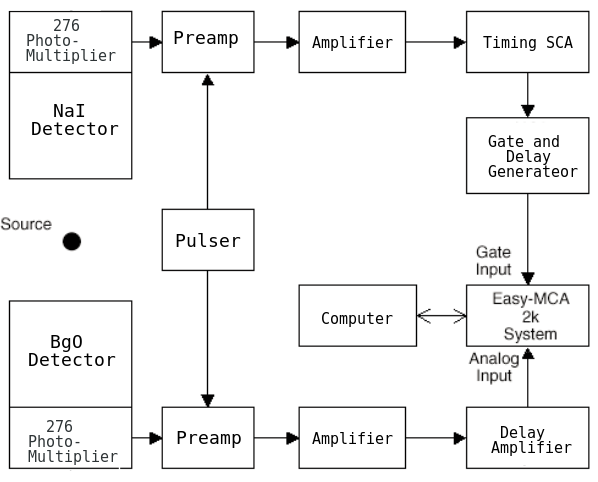
\includegraphics[width=.45\textwidth]{Figures/gamma_coin_circuitry.png}
    \caption{Circuitry behind the detectors used to measure gamma coincidence
    (Inspired by \cite{Experiment_Set_Up:1}).}
    \label{figure:circuitry}
\end{figure}
%Figure 2
\begin{figure}[H]
     \centering
     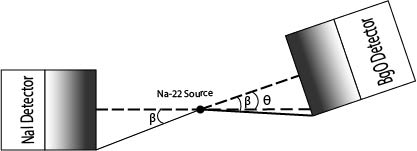
\includegraphics[width=.45\textwidth]{Figures/detector_set_up.jpg}
     \caption{Set up of angular variation between the two detectors and the
     \textsuperscript{22}Na source (inspired by \cite{Experiment_Set_Up:2}).}
     \label{figure:set_up}
\end{figure}
%Figure 3
\begin{figure}[H]
    \centering
    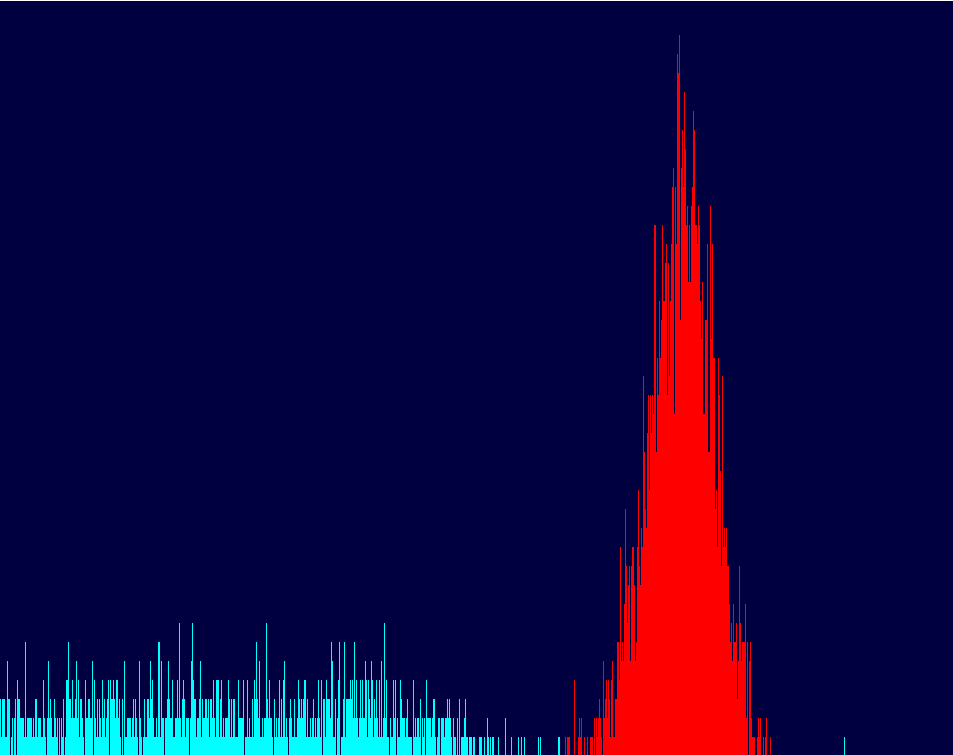
\includegraphics[width=0.9\linewidth]{Figures/sample_spectrum.png}
    \caption{Spectrum produced with the detectors 15 cm and 0 degrees offset
    from the source. Peak highlighted was integrated for count rate.}
    \label{figure:spectrum}
\end{figure}
%Figure 4, 5, & 6
\begin{figure}[H]
    \centering
    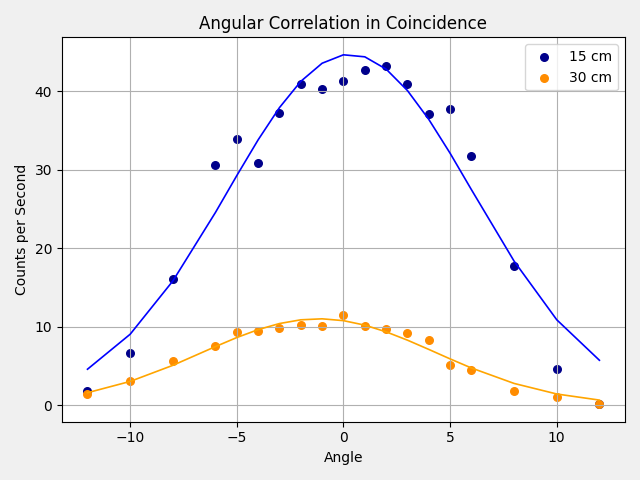
\includegraphics[width=0.45\textwidth]{Figures/coincidence_gauss_fit.png}
    \caption{Table \ref{table:model1_table} visualized and fitted with a Gaussian
    function.}
    \label{figure:model1_graph}
    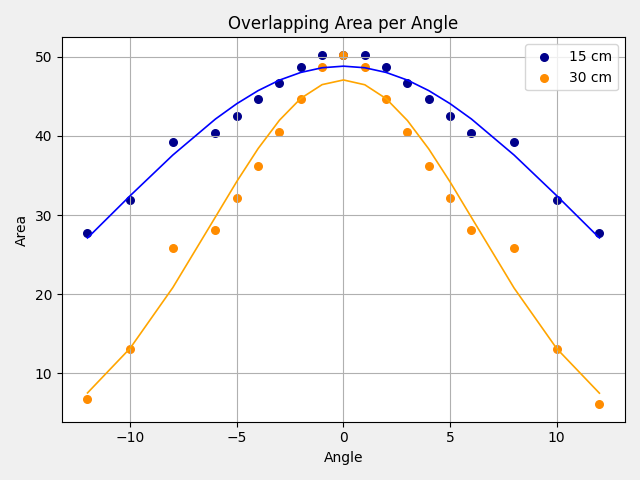
\includegraphics[width=0.45\textwidth]{Figures/overlapping_area_gauss_fit.png}
    \caption{Table \ref{table:model2_table} visualized and fitted with a Gaussian
    function.}
    \label{figure:model2_graph}
    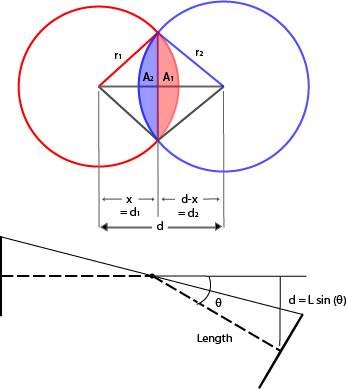
\includegraphics[width=0.45\textwidth]{Figures/geometry.jpg}
    \caption{Set up of the geometry used to derive the correlation between
    overlapping area and angular offset (inspired by \cite{Geometry}).}
    \label{figure:geometry}
\end{figure}
\newpage

\printbibliography

\end{document}
